\documentclass[aps, twocolumn, floatfix, superscriptaddress]{revtex4}
\usepackage{amsmath, amssymb, amsfonts, gensymb}
\bibliographystyle{apsrev}
\usepackage{graphicx}
\graphicspath{ {Figures/} }
\newcommand{\tdc}[3][]{\frac{\mathrm{d}^{#1}#2}{\mathrm{d}#3^{#1}}} % total differential change.
\newcommand{\pdc}[3][]{\frac{\partial^{#1} #2}{\partial #3^{#1}}} % partial differential change.
\newcommand{\td}[1]{\mathrm{d}#1}
\newcommand{\pd}[1]{\partial#1}

\begin{document}

\title{Hydrodynamics of a Self-propelled C-boat}

\author{V. S. Akella}
\affiliation{Collective Interactions Unit, OIST Graduate University, 1919-1 Tancha, Onna-son, Okinawa, Japan 904-0495}
\author{D. K. Singh}
\affiliation{Collective Interactions Unit, OIST Graduate University, 1919-1 Tancha, Onna-son, Okinawa, Japan 904-0495}
\author{S. Mandre}
\affiliation{School of Engineering, Brown University, 182 Hope Street, Providence, RI 02906, USA}
\author{M. M. Bandi}
\affiliation{Collective Interactions Unit, OIST Graduate University, 1919-1 Tancha, Onna-son, Okinawa, Japan 904-0495}
\email[Corresponding Author: ]{bandi@oist.jp}

\date{\today}

\begin{abstract}
In the present work, we attempt to understand the dynamics of a \emph{c-boat} at the air-water interface. A \emph{c-boat} is a disc-shaped agarose gel tablet with all the water in the agarose gel replaced by camphoric acid. Camphoric acid spreads over the air-water interface due to the interfacial tension forces creating concentration gradients which in turn cause the interfacial tension gradients around the c-boat. The asymmetry in the interfacial tension gradients spontaneously set the c-boat in motion at the air-water interface. Furthermore, we observe three different modes of motion, namely continuous, harmonic and periodic, due to the evaporation/sublimation of camphoric acid. We explain these modes in terms of ratio of two time scales, $\tau_{\eta}$ and $\tau_{\sigma}$, where $\tau_{\eta}$ is the time required for the development of Marangoni forces to overcome the viscous forces and $\tau_{\sigma}$ is the time during which Marangoni forces dominate the viscous forces. The continuous, harmonic and periodic motions are observed when $\frac{\tau_{\eta}}{\tau_{\sigma}} \approx 1$,  $\frac{\tau_{\eta}}{\tau_{\sigma}} >~ 1$ and $\frac{\tau_{\eta}}{\tau_{\sigma}} >> 1$ respectively. Experimentally, the ratio of the time scales is varied by changing the interfacial tension of the air-water interface using Sodium Dodecyl Sulfate (SDS).
\end{abstract}

\maketitle
\section{Introduction}
\section{Experimental Section}

\section{Dynamic C-boat}
When the c-boat is placed at the air-water interface, the following processes lead to the movement of c-boat on the air-water interface.
\begin{itemize}
\item Camphoric acid spreads onto the air-water interface via two processes. 1. Interfacial forces draw the camphoric acid molecules out of the c-boat to minimize the interfacial energy. 2. Diffusion of camphoric acid molecules onto the air-water interface. Dissolution is another mechanism by which camphoric acid is drawn out of c-boat but it is very minimal as the solubility of camphoric acid is $\approx$ 40 mM at 25 \celsius.
\item As mentioned earlier, camphoric acid is a surface active molecule and lowers the air-water interfacial energy. When a c-boat is introduced at the air-water interface, the out-flux of camphoric acid molecules from the c-boat sets up interfacial tension gradients symmetrically around the c-boat. A random perturbation arising due to change in local temperature or contamination of air-water interface due to unavoidable dust particles in air spontaneously break the symmetric interfacial tension gradients around the c-boat. When the perturbation is strong enough to overcome the viscous drag forces on the c-boat, the c-boat starts moving. Once the c-boat starts moving it further enhances the asymmetry resulting in continuous motion of the c-boat.
\item The air-water interface never gets saturated with the camphoric acid because camphoric acid sublimes into room. Therefore the motion of the c-boat lasts as long as there is camphoric acid in the c-boat.
\end{itemize}
\subsection{Lifetime of a C-boat}
\label{sec:lifetime}
The forces acting on the c-boat are, 1. Marangoni forces set up by the interfacial tension gradients which are in turn caused camphoric acid concentration gradients, 2. Drag forces due to the viscosity of the medium. During the course of the experiment, camphoric acid sublimes into the surroundings resulting in decrease in Marangoni forces. Another mechanism that affects the lifetime of a c-boat is: the dissolution of camphoric acid in water which decreases the background air-water interfacial tension resulting in lesser interfacial tension gradients. However, the amount of camphoric acid in a c-boat ($\simeq 7\ \mathrm{mg}$) is negligibly small to modify the interfacial tension of water by a measurable amount. The interfacial tension of water, when saturated with camphoric acid ($\simeq 8\ \mathrm{g/l}$), is $\simeq 60\ \mathrm{dy/cm}$. As camphoric acid sublimes the physical characteristics of the system change continuously. Figure~\ref{fig:lifetime} is the speed of a c-boat as function of time. 
\begin{figure}[ht]
    \begin{center}
       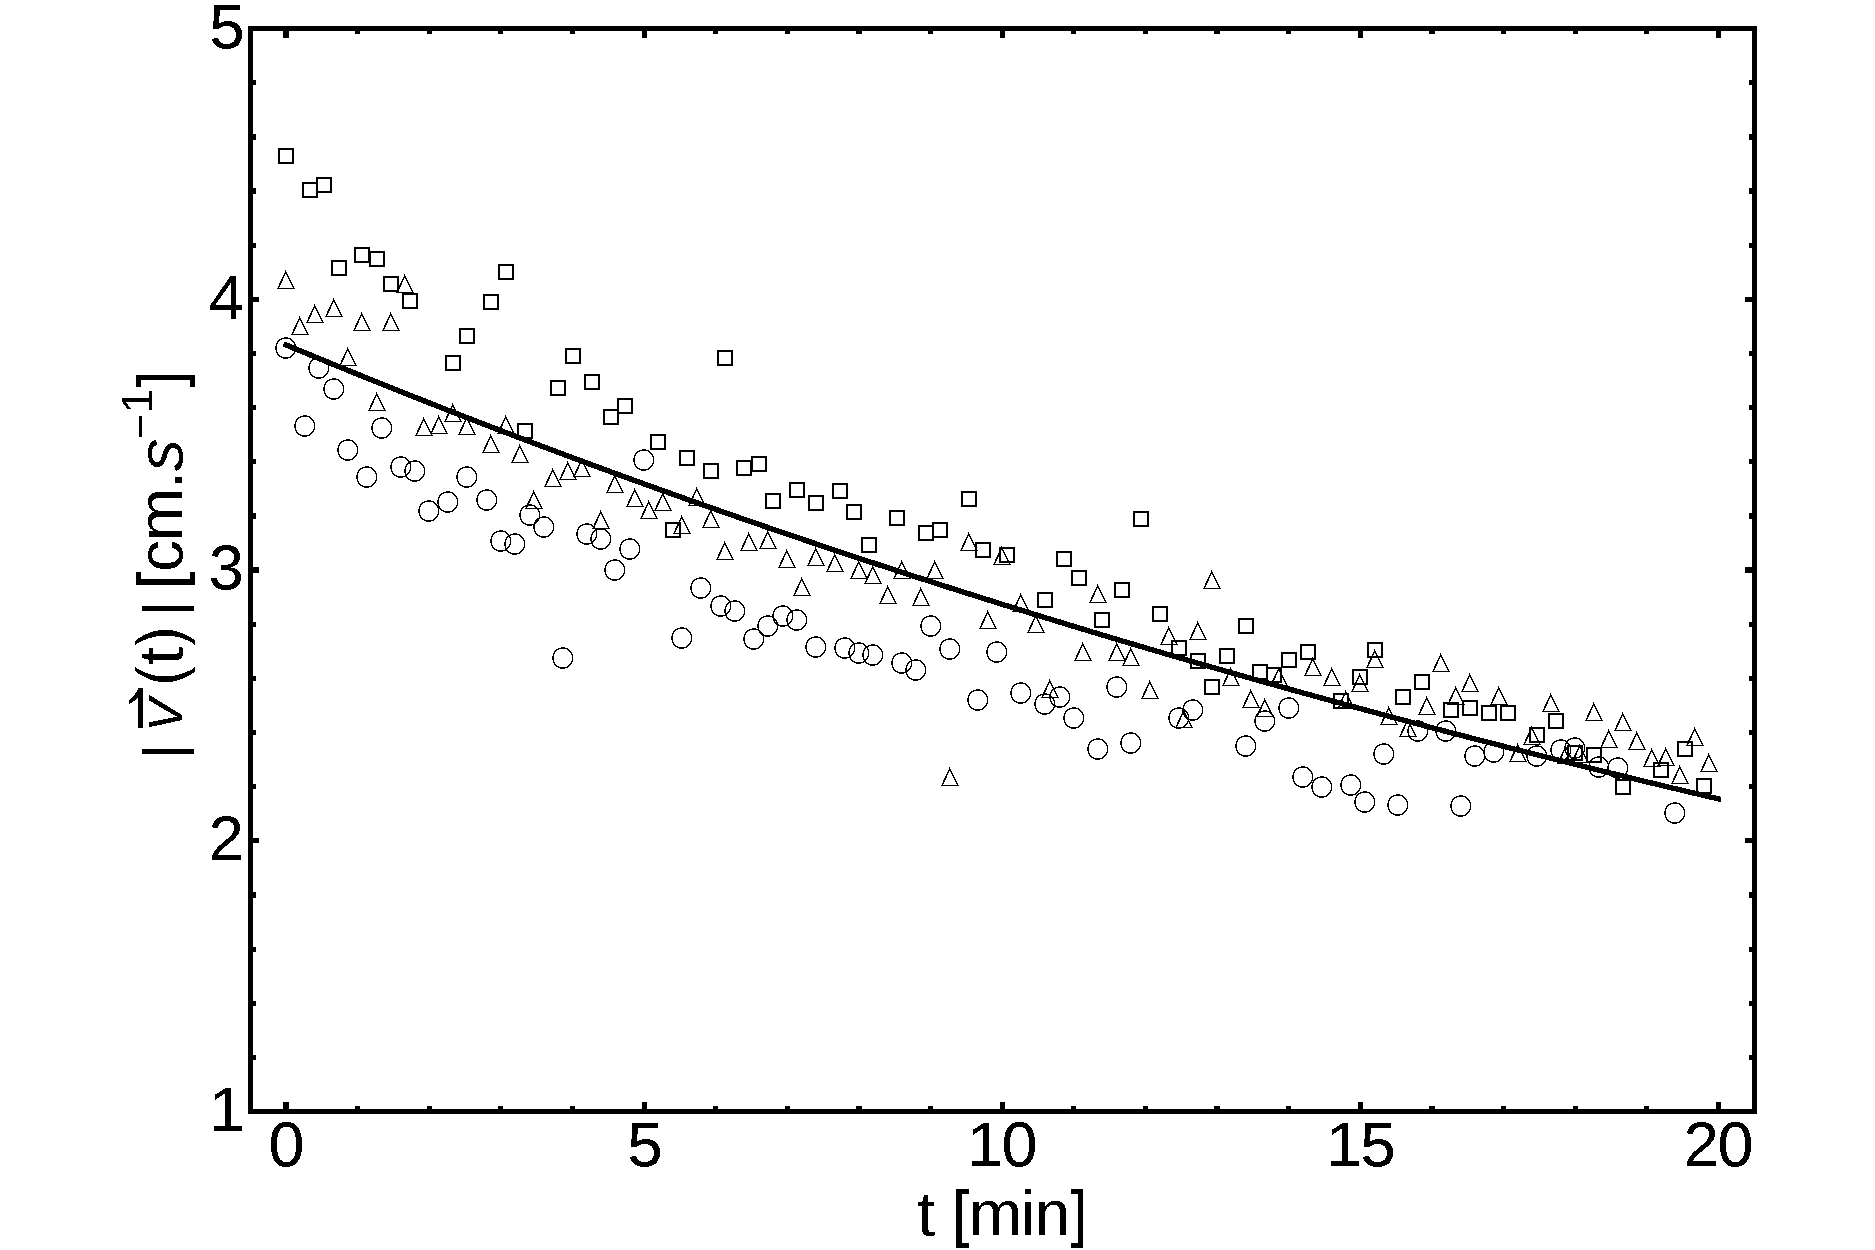
\includegraphics[scale=0.25]{figure6.pdf}
    \end{center}
    \caption{Lifetime of the c-boat.}
    \label{fig:lifetime}
\end{figure}
\subsection{Oscillatory Motion of the C-boat}
\label{sec:movingc-boat}
Another interesting phenomenon observed in c-boat dynamics is the oscillatory motion of the c-boat. Figure~\ref{fig:absvnosds} shows the time traces of the c-boat speed at different intervals and the corresponding power spectra. At the beginning of the experiment there is a strong peak at $\approx 1\ \mathrm{Hz}$ in the power spectrum. However the peak completely disappears at long times. The observed phenomenon is shown in figure~\ref{fig:absvnosds}.   
\begin{figure}[ht]
    \begin{center}
       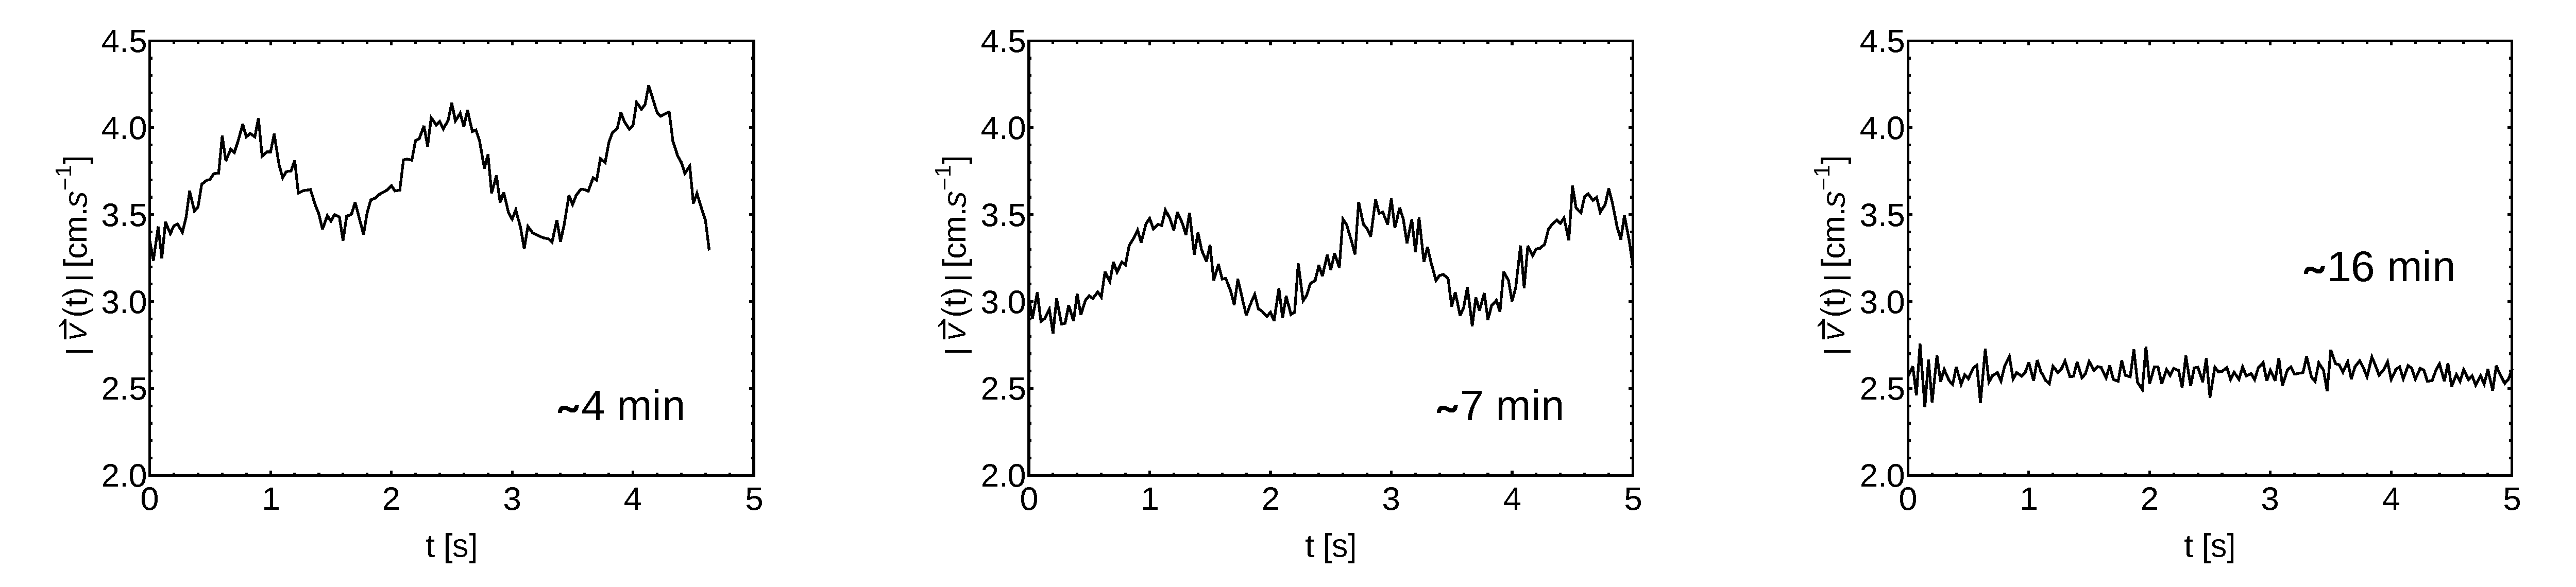
\includegraphics[scale=0.1]{figure7.pdf}
    \end{center}
    \caption{(a) Oscillation in speed of the c-boat at different intervals. (b) The power spectrum of speed.}
    \label{fig:absvnosds}
\end{figure}
The motion of c-boat involves two processes. 1. At an instant position of the c-boat on the air-water interface, Marangoni forces are established because camphoric acid spreads and creates interfacial tension gradients around the c-boat and 2. The Marangoni forces propel the c-boat to a new position where the interfacial tension (concentration of camphoric acid) is high (low). At the new position, the same processes repeat and the c-boat continues to move. Let us define $\tau_{\gamma}$ as the time required to establish sufficient Marangoni forces to overcome the drag forces and $\tau_{\lambda} = \frac{\|\vec{u}\|}{\lambda}$ as the time required for the c-boat to move a distance, $\lambda$ defined as the maximum distance, measured from the center of the c-boat, to which camphoric acid spreads without subliming/evaporating. The c-boat motion can be continous, oscillatory or intermittent when $\tau_{\gamma} < \tau_{\lambda}$, $\tau_{\gamma} \approx \tau_{\lambda}$ or $\tau_{\gamma} > \tau_{\lambda}$ respectively. From the measurements in section~\ref{sec:caspread}, the radius of influence of the c-boat is $\approx 3.6\ \mathrm{cm}$ for a 3 $\mathrm{mm}$ diameter c-boat. Furthermore, the average distance travelled by the c-boat during a period of oscillation ($\approx 1\ \mathrm{Hz}$) is also $\approx$ 3.6 $\mathrm{cm}$. This observation indicates that, the c-boat always moves from one position to another position in steps of $\lambda$ however, the motion appears to be continuous, oscillatory or intermittent depending on $\tau_{\gamma}$ and $\tau_{\lambda}$. A typical c-boat dynamics experiment, with a 3 $\mathrm{mm}$ diameter c-boat, is recorded for 20 minutes during which we observed the oscillatory and continuous motions as shown in figure~\ref{fig:absvnosds}. During the course of the experiment, camphoric acid sublimes into the surroundings resulting in continuous decrease in $\lambda$ of the c-boat, thereby increasing $\tau_{\lambda}$. Therefore, the transistion from $\tau_{\gamma} \approx \tau_{\lambda}$ to $\tau_{\gamma} < \tau_{\lambda}$ leads to oscillatory to continuous motion of the c-boat. Further, to experimentally verify the above hypothesis we used Sodium Dodecyl Sulfate (SDS) to modify the interfacial tension of air-water interface. From equation~\ref{eq:jensen}, modifying the background interfacial tension slows down rate of camphoric acid spread on the air-water interfaction thereby increasing $\tau_{\gamma}$. When the interfacial tension is sufficiently modified, the system goes into $\tau_{\gamma} > \tau_{\lambda}$ regime exhibiting the intermittent motion of the c-boat. Figure~\ref{fig:absvsds} shows the intermittent, oscillatory and continuous regimes at different concentrations of SDS.
\begin{figure}[ht]
    \begin{center}
       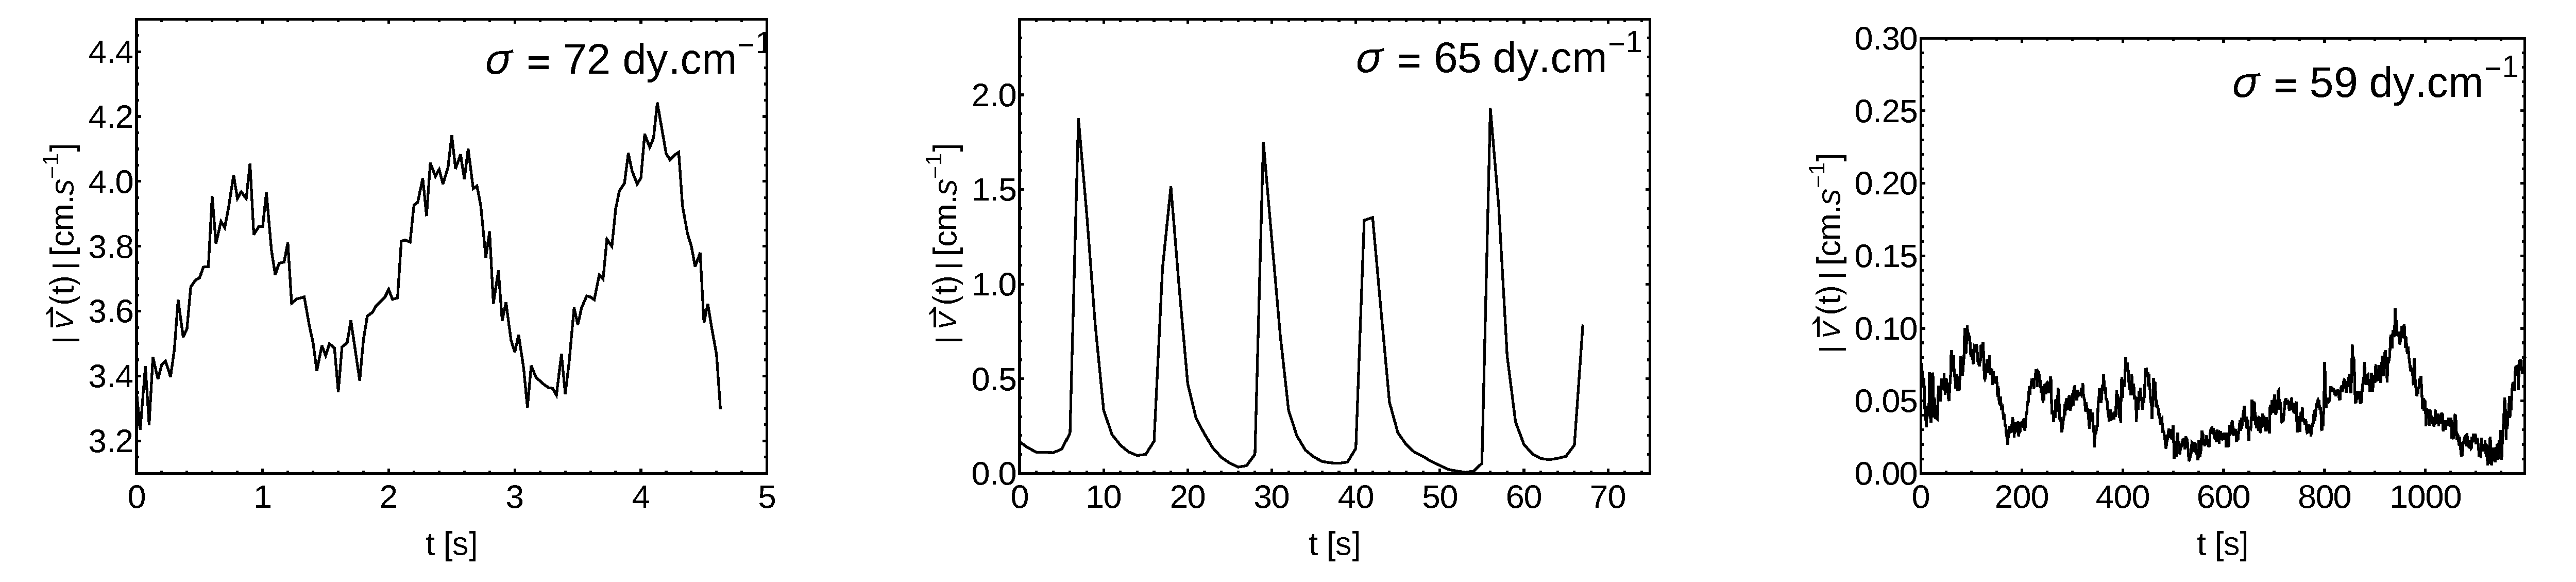
\includegraphics[scale=0.1]{figure8.pdf}
    \end{center}
    \caption{(a) Oscillations in the speed of the c-boat at different concentrations of Sodium Dodecyl Sulfate (SDS) (b) The power spectrum of speed.}
    \label{fig:absvsds}
\end{figure}
\section{Model for Dynamic C-boat}
\begin{align}
\pdc{}{t}c(x, t) &= \mathrm{D} \pdc[2]{}{x}c(x, t) - \tdc{x}{t} \pdc{}{x}c(x, t)  - \xi c(x, t) \\
m\tdc[2]{x}{t} &= -\eta \tdc{x}{t} + \zeta \tdc{}{x}c(x,t) 
\end{align}
This is requiring hell lot of changes.
VSA, DKS, SB and MMB were supported by the OIST Graduate University with subsidy funding from the Cabinet Office, Government of Japan. RKS was hosted by OIST Graduate University on a research internship while performing this work. MMB acknowledges L. Mahadevan for introducing the camphor boat system and subsequent scientific discussions, and D. Vu Anh for help with preliminary experiments.

\section{Summary}
\label{sec:summary}


\acknowledgments
VSA, DKS, SB and MMB were supported by the OIST Graduate University with subsidy funding from the Cabinet Office, Government of Japan. RKS was hosted by OIST Graduate University on a research internship while performing this work. MMB acknowledges L. Mahadevan for introducing the camphor boat system and subsequent scientific discussions, and D. Vu Anh for help with preliminary experiments.

\bibliography{all}

\end{document} 
